\chapter{Evaluation}\label{chap:evaluation}

% --------------------- Section 1 ---------------------

\section{Introduction}\label{sec:evaluation-introduction}
To validate the utility of stable specialization, we conducted a series of experiments focusing on ecosystem analysis.
These evaluations aimed to identify real-world scenarios where stable specialization could provide significant benefits, particularly in terms of code maintainability.
The experiments were designed to analyze a diverse set of public Rust codebases, examining their use of traits and generic programming patterns.
By applying our specialization technique to these codebases, we sought to demonstrate its practical applicability and effectiveness in real-world scenarios.

\paragraph{Approach}
To conduct the experiments, we developed a static analysis tool that scans the selected Rust codebases for instances of the identified patterns, which we'll show later.
More specifically, we instructed the compiler to build a custom AST starting from the HIR for each function (including trait and impls fn items) in the codebase.

After building the AST, using an heuristic we grouped together functions that could be specializable between one another.
To do so, we used a naming-based heuristic combined with a same-number-of-parameters check.
For example, if we had a function named \texttt{process\_int} taking an \texttt{i32} parameter and another function named \texttt{process\_float} taking an \texttt{f32} parameter, we would group them together as they likely represent specialized versions of a more generic function.
We also split the functions based on their origin (bare function, trait items, impl items) and if they were associated with a trait, we used another similar heuristic for the two traits.

Once we had these groups, we calculated the tree edit distance of each function in the group to one another.
This was done using the ZSS algorithm~\cite{ZSSTreeEditDistance89}, which computes the minimum number of operations required to transform one tree into another, allowing us to quantify the structural similarity between functions' ASTs.
The ZSS algorithm has a worst-case complexity of \(O(n^4)\), where \(n\) is the number of nodes in the larger tree, which makes it suitable for our analysis of function ASTs, but also computationally intensive for larger trees, which explains some of the longer analysis times we had.
After calculating the edit distance, we got the similarity by using this formula $$1 - \frac{\text{dist}}{\text{max\_size}}$$ where \texttt{dist} is the tree edit distance between the two functions and \texttt{max\_size} is the size of the largest AST between the two.

Finally, we filtered out groups that had an average similarity lower than a certain threshold to focus on the most promising candidates for specialization.
We also made sure to add a further optimization to avoid analyzing trees that had way too different sizes, as they would mathematically never reach a good enough similarity score, using the following formula $$\frac{\text{min\_size}}{\text{max\_size}} < \text{threshold}$$ where \texttt{min\_size} is the size of the smallest AST between the two and \texttt{threshold} is the similarity threshold set for the analysis.

This approach allowed us to systematically identify potential specialization opportunities across a wide range of Rust codebases, providing a solid foundation for evaluating the effectiveness of stable specialization in real-world scenarios.
It's important to note that our analysis was based on heuristics to identify the relevant patterns and the specialization opportunities within the selected codebases.
As such, there is a possibility that some patterns were overlooked or misclassified, which could affect the comprehensiveness of our findings.
It's also important to note that not all instances where specialization is possible it should be applied, e.g.\@ if the specialized versions do not provide significant performance improvements or if they complicate the code unnecessarily, like adding more boilerplate than they would reduce.

\paragraph{Analysis Setup}
The analysis was performed on a machine with an Intel Core i7-8565U 4-Core 8-Thread Processor and 16 GB of RAM, running Ubuntu 24.04 LTS.
The Rust toolchain used for the analysis was  nightly-2025-11-17, with our static analysis tool integrated into the compiler as a custom pass.
The analysis was executed starting from November 17, 2025 and to ensure a comprehensive evaluation, it got run with two different similarity thresholds:
\begin{itemize}
	\item \textbf{90\% Similarity Threshold}: This threshold was chosen to capture a broader range of specialization opportunities, allowing for more structural differences between functions while still identifying meaningful similarities.
	\item \textbf{99\% Similarity Threshold}: This higher threshold was selected to focus on functions that are nearly identical in structure, ensuring that only the most closely related functions were considered for specialization.
\end{itemize}
These thresholds allowed us to evaluate the effectiveness of stable specialization across different levels of similarity, providing insights into its applicability in various scenarios.

\paragraph{Project Selection}
An important step to conduct this research was to select a set of representative Rust projects from the open-source ecosystem.
For this purpose, we selected some of the most downloaded crates from \texttt{crates.io} as well as some popular projects and other less known ones, ranging from code editors to broadly used libraries, ensuring that our analysis captures a diverse set of programming patterns and practices.
The analyzed projects are listed in Table~\ref{tab:analysis-projects}, along with some relevant metadata such as their GitHub stars, \texttt{crates.io} dependents and downloads and the total number of functions and traits found while analyzing the projects.

\paragraph{Pattern Identification}
To keep the analysis focused and feasible and to ensure that we could draw meaningful conclusions from the results, we concentrated on identifying specific patterns that are likely to benefit from stable specialization.
These patterns include:
\begin{itemize}
	\item \textbf{Manual Dispatch}: In the trait we have a version of the function for each type we want to support and when calling the function, we manually dispatch to the correct version, e.g.\@ in Listing~\ref{fig:manual-dispatch}.
	\item \textbf{Monomorphized Traits}: A trait is defined for each type we want to support and each implementation provides a specialized version of the function, requiring the caller to manually select the correct trait, e.g.\@ in Listing~\ref{fig:monomorphized-traits}.
	\item \textbf{Standalone Functions}: A standalone function is defined for each type we want to support and the caller is responsible for calling the correct version, e.g.\@ in Listing~\ref{fig:standalone-functions}.
	\item \textbf{Inherent Impls}: A struct has inherent implementations for each type we want to support, providing specialized versions of the function, e.g.\@ in Listing~\ref{fig:inherent-impls}.
\end{itemize}
Other than these, we've also pointed out some additional patterns that we did not include in the analysis because they were less common or harder to analyze in a systematic way, such as:
\begin{itemize}
	\item \textbf{Type Level Dispatch}: A wrapper structure is created to hold the type and the value we want to specialize on, and then we implement the trait for each disjunct specialized version of the wrapper structure, e.g.\@ in Listing~\ref{fig:type-level-dispatch}. This does not support default implementations.
	\item \textbf{Macros}: Macros are used to generate specialized implementations based on the input type, which reduces boilerplate but does not support default implementations.
	\item \textbf{Pattern matching blocks}: Pattern matching is used to select the appropriate code path based on the type or value.
	\item \textbf{If blocks}: Conditional statements are used to select the appropriate code path based on the type or value.
\end{itemize}
The baseline implementations using unstable specialization and \mytool{} specialization can be seen in Listings~\ref{fig:unstable-specialization} and ~\ref{fig:tool-specialization} respectively.
For each of the patterns shown in the listings, we created a minimal example that demonstrates how the pattern works and the call to the default function.
To call the specialized version (in the examples always the one for \texttt{i32}), for all Listings~\ref{fig:tool-specialization} to~\ref{fig:monomorphized-traits}, we'd need some more complex logic to check the type and call the correct specialized version, which could look similar to what's shown in Listing~\ref{fig:call-check-type}.
For Listing~\ref{fig:type-level-dispatch}, the default implementation is not supported, but the call doesn't need any type check as the correct specialized version is selected at compile time based on the type of the wrapper structure.

\begin{figure}[htbp!]
	\centering
	\showrust[0.98\linewidth]{experimentation-call-check-type.rs}
	\captionsetup{type=listing,skip=2pt}
	\caption{Example of the type check to select the correct specialized version}
	\label{fig:call-check-type}
\end{figure}

It's important to note that even though each of these patterns could be implemented using stable specialization, some patterns are more likely to benefit from it than others.
Firstly, for all patterns stable specialization would completely remove the method call boilerplate needed to select the correct specialized version, which as we've seen in Listing~\ref{fig:call-check-type} can be quite verbose and error-prone.
Secondly, some patterns inherently introduce more complexity and boilerplate than others, making them more suitable candidates for stable specialization, like the \textbf{Monomorphized Traits} and \textbf{Manual Dispatch} patterns, which would also benefit from the removal of a whole trait and trait fn respectively.
A summary of patterns shown in Listings~\ref{fig:tool-specialization} to~\ref{fig:type-level-dispatch} are reported in Table~\ref{tab:code-reduction-estimates}, where we also estimated the code reduction that stable specialization would provide for each pattern compared to their baseline implementations.
Anyways, we believe that stable specialization could provide significant benefits across all these patterns by reducing boilerplate (as we've just discussed), improving performance and enhancing code readability and maintainability.
Furthermore, many of these patterns do not support certain specialization features, like specialization based purely on trait bounds or default implementations.
By leveraging stable specialization, developers can achieve more efficient and maintainable code across a variety of programming patterns.

\begin{figure}[htbp!]
	\centering
	\begin{minipage}{0.49\textwidth}
		\centering
		\showrust[0.98\linewidth]{experimentation-unstable.rs}
		\captionsetup{type=listing,skip=2pt}
		\caption{Unstable Specialization}
		\label{fig:unstable-specialization}
	\end{minipage}
	\hfill
	\begin{minipage}{0.49\textwidth}
		\centering
		\showrust[0.98\linewidth]{experimentation-tool.rs}
		\captionsetup{type=listing,skip=2pt}
		\caption{\mytool{} Specialization}
		\label{fig:tool-specialization}
	\end{minipage}
\end{figure}

\begin{figure}[p!]
	\centering
	\begin{minipage}{0.48\textwidth}
		\centering
		\begin{minipage}{\linewidth}
			\centering
			\showrust[0.98\linewidth]{experimentation-standalone-functions.rs}
			\captionsetup{type=listing,skip=5pt}
			\caption{Standalone Functions}
			\label{fig:standalone-functions}
		\end{minipage}

		\vspace{2em}

		\begin{minipage}{\linewidth}
			\centering
			\showrust[0.98\linewidth]{experimentation-inherent-impls.rs}
			\captionsetup{type=listing,skip=5pt}
			\caption{Inherent Impls}
			\label{fig:inherent-impls}
		\end{minipage}

		\vspace{2em}

		\begin{minipage}{\linewidth}
			\centering
			\showrust[0.98\linewidth]{experimentation-manual-dispatch.rs}
			\captionsetup{type=listing,skip=5pt}
			\caption{Manual Dispatch}
			\label{fig:manual-dispatch}
		\end{minipage}
	\end{minipage}
	\hfill
	\begin{minipage}{0.48\textwidth}
		\centering
		\begin{minipage}{\linewidth}
			\centering
			\showrust[0.98\linewidth]{experimentation-monomorphized-traits.rs}
			\captionsetup{type=listing,skip=5pt}
			\caption{Monomorphized Traits}
			\label{fig:monomorphized-traits}
		\end{minipage}

		\vspace{2em}

		\begin{minipage}{\linewidth}
			\centering
			\showrust[0.98\linewidth]{experimentation-type-level-dispatch.rs}
			\captionsetup{type=listing,skip=5pt}
			\caption{Type Level Dispatch}
			\label{fig:type-level-dispatch}
		\end{minipage}
	\end{minipage}
\end{figure}

% --------------------- Section 2 ---------------------

\section{Results}\label{evaluation-results}
The analysis was run with a similarity threshold of 90\% and 99\% and the results for the two are reported in Tables~\ref{tab:results-90} and~\ref{tab:results-99} respectively.
For each project and threshold, we reported its analysis time in seconds, peak RSS in MB, number of unique specializable functions, from which is also reported the percentage of the total project's functions and the same is then done for unique traits and percentages.

\begin{wrapfigure}{r}{0.4\linewidth}
	\centering
	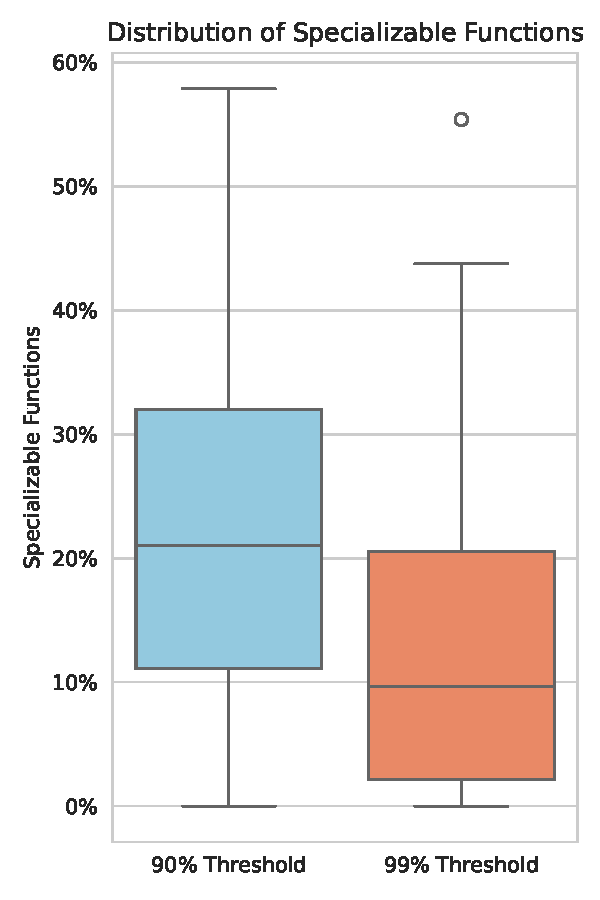
\includegraphics[width=0.38\textwidth]{figs/specializable_functions_distribution_box_plot.pdf}
	\captionsetup{type=figure,skip=2pt}
	\caption{Distribution of Spec. Fns}
	\label{fig:distribution-specializable-functions}
\end{wrapfigure}
The findings of our experimentation revealed several interesting insights into the prevalence and effectiveness of stable specialization in real-world Rust codebases.
Across the analyzed projects, we identified numerous instances where stable specialization could be applied to reduce boilerplate code and improve performance.
As shown in Figure~\ref{fig:distribution-specializable-functions}, an average of more than 20\% of functions in the analyzed codebases were found to be specializable at 90\% similarity threshold, with some projects exhibiting even higher proportions.
At 99\% similarity threshold, the average was around 10\%, indicating that even with stricter similarity requirements a significant number of functions could benefit from specialization.

As expected based on our initial hypotheses, the major results are in projects that heavily utilize traits and generics.
We also found that as the number of functions and traits in a project increases, so does the percentage of specializable instances, indicating that larger codebases stand to benefit significantly from stable specialization, as we can see in Figure~\ref{fig:correlation-functions-specializable}.
\begin{figure}[htbp!]
	\centering
	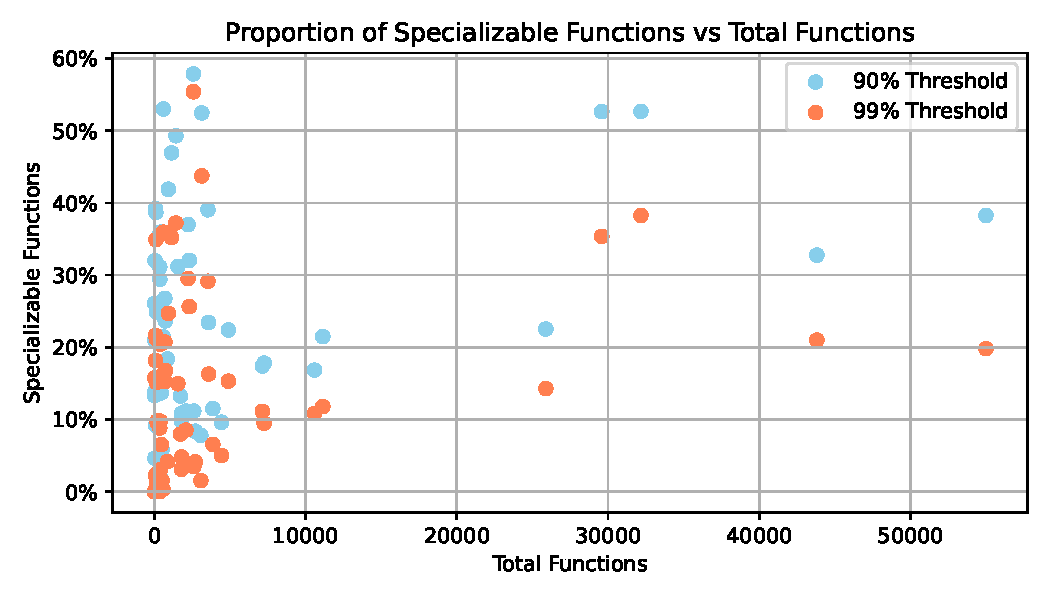
\includegraphics[width=0.75\textwidth]{figs/proportion_specializable_functions.pdf}
	\captionsetup{type=figure,skip=2pt}
	\caption{Correlation between Number of Functions and Spec. Functions}
	\label{fig:correlation-functions-specializable}
\end{figure}

\begin{wrapfigure}{l}{0.4\linewidth}
	\centering
	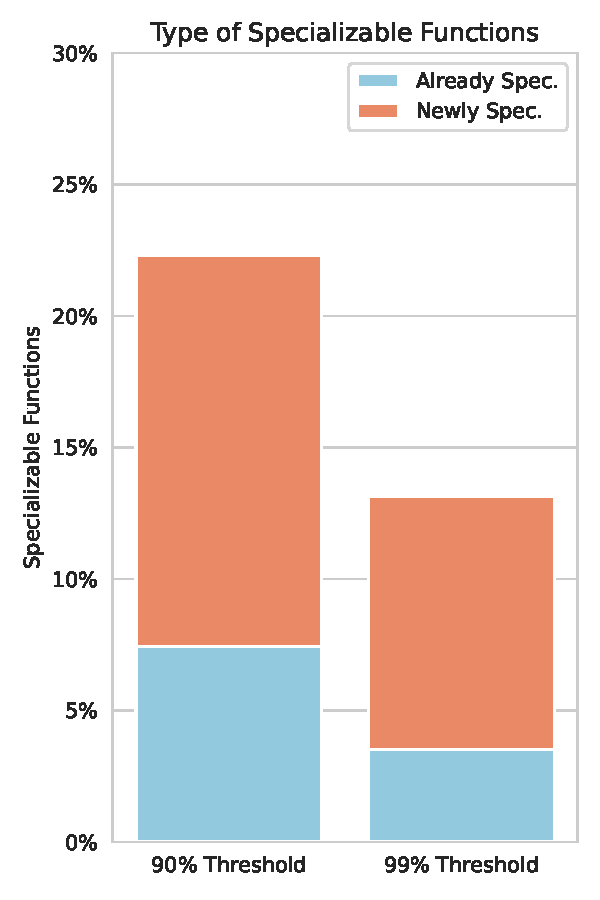
\includegraphics[width=0.38\textwidth]{figs/specializable_functions_bar_chart.pdf}
	\captionsetup{type=figure,skip=2pt}
	\caption{Types of Spec. Fns}
	\label{fig:specializable-functions-already-vs-newly}
\end{wrapfigure}
We then also set to understand the impact of a full stable specialization implementation versus the current subset of non-overlapping specialization that Rust offers.
To do so, we identified already specializable functions as functions that satisfy our specializability heuristic defined earlier and that have a permutation of their type parameters that makes them non-overlapping.
Newly specializable functions are instead functions that satisfy our heuristic but do not have any permutation of their type parameters that makes them non-overlapping and thus could only be specialized using a full stable specialization implementation.
Overlap can be caused by multiple factors, such as the presence of generic type parameters, trait bounds that are not mutually exclusive or more simply equal types used in different functions.
For example \texttt{fn a(x:\@ i32, y:\@ u32)} is already specializable with \texttt{fn b<T>(x:\@ T, y:\@ u32)}, because function \texttt{b}'s parameters could be permuted into a non-overlapping \texttt{fn b2<T>(y:\@ u32, x:\@ T)}, whatever type \texttt{T} ends up being.
As shown in Figure~\ref{fig:specializable-functions-already-vs-newly}, in both analysis we found that a full stable specialization implementation could on average triple the number of functions available for specialization compared to the current Rust specialization capabilities, highlighting the significant potential of specialization.
In particular, at 90\% similarity threshold, we found that on average around 67\% of specializable functions were newly specializable using stable specialization, while at 99\% similarity threshold, this proportion was around 73\%.

\begin{wrapfigure}{r}{0.4\linewidth}
	\centering
	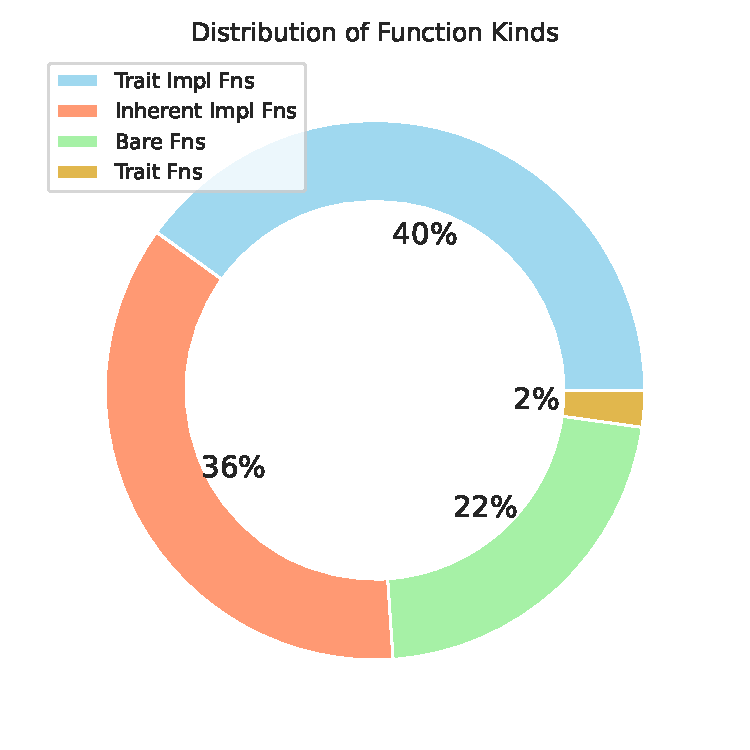
\includegraphics[width=0.38\textwidth]{figs/functions_kind_pie.pdf}
	\captionsetup{type=figure,skip=2pt}
	\caption{Types of Fns}
	\label{fig:functions-by-kind}
\end{wrapfigure}
Afterwards, we also tried to understand which of the patterns we identified earlier were the most common in the analyzed codebases.
To do this, we first divided the functions into four distinct categories based on their structure: bare functions (not associated with any trait or impl), trait functions (defined within a trait), trait impl functions (defined within a trait impl block) and inherent impl functions (defined within an inherent impl block).
As shown in Figure~\ref{fig:functions-by-kind}, we found that the majority of functions in the analyzed codebases were trait impl functions, followed by inherent impl functions and bare functions, with trait functions being by far the least common.
As Figure~\ref{fig:distribution-function-kinds} shows, we found that the group with the majority of specializable functions were trait impl functions, indicating that these functions were not only the most common but also the most likely to benefit from stable specialization.
In particular, the most common patterns associated to trait impls are the \textbf{Monomorphized Traits} and \textbf{Manual Dispatch} patterns, hinting that many developers resort to these approaches to achieve specialization in their code.
These two patterns, as seen earlier, are also the ones that would benefit the most from stable specialization, as they would both see a significant reduction in boilerplate code and complexity, even more so than other patterns.
By applying stable specialization, we could achieve significant reductions in code complexity and improved maintainability.
\begin{figure}[htbp!]
	\centering
	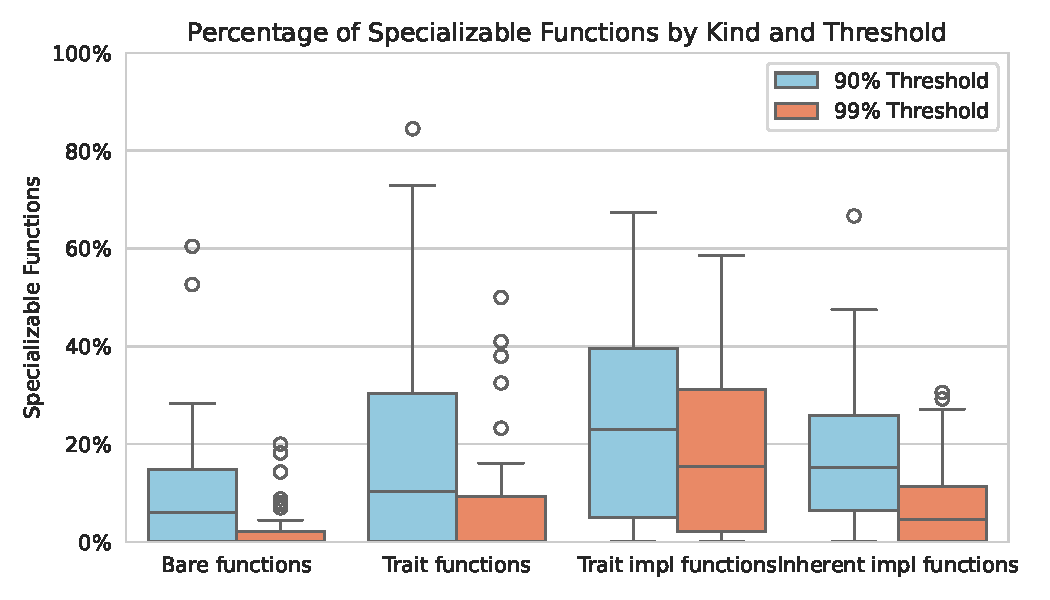
\includegraphics[width=0.75\textwidth]{figs/specializable_functions_box_plot.pdf}
	\captionsetup{type=figure,skip=2pt}
	\caption{Distribution of Spec. Functions by Kind}
	\label{fig:distribution-function-kinds}
\end{figure}

Furthermore, stable specialization could effectively handle default implementations and specialization based purely on trait bounds, which are not supported by many of the existing patterns.
This capability allows developers to write more generic and reusable code without sacrificing performance.

Overall, our experimentation demonstrated that stable specialization is a valuable tool for Rust developers, offering a practical solution to common challenges associated with generic programming and code specialization.

% --------------------- Section 3 ---------------------

\section{Considerations}\label{sec:evaluation-considerations}
While our evaluation has yielded promising results regarding the potential benefits of stable specialization in Rust codebases, there are several important considerations to keep in mind when interpreting these findings.

Firstly, it's crucial to recognize that not all instances of specializable functions necessarily warrant specialization.
The decision to specialize a function should be based on a careful evaluation of the trade-offs involved, including potential performance gains, code complexity and maintainability.
In some cases, the overhead of specialization may outweigh the benefits, particularly if the specialized versions do not provide significant performance improvements or if they complicate the code unnecessarily.
Therefore, developers should exercise discretion when applying stable specialization, ensuring that it aligns with the specific needs and goals of their projects.

Secondly, our analysis was based on heuristics to identify specializable functions and patterns within the selected codebases.
As such, there is a possibility that some patterns were overlooked or misclassified, which could affect the comprehensiveness of our findings, potentially yielding false positives or negatives.
Future work could involve refining these heuristics or employing more sophisticated analysis techniques to enhance the accuracy of the identification process.

One could also argue that this analysis shows the poor quality of some Rust codebases, as they resort to patterns that introduce boilerplate and complexity.
While this may be true in some cases, it's important to note that as shown in Figure~\ref{fig:specializable-functions-already-vs-newly} the majority of the identified specializable functions could not be specialized using current Rust capabilities due to overlapping implementations.
This indicates that even well-written codebases could benefit from stable specialization, as it provides a more flexible and powerful mechanism for achieving specialization without the limitations imposed by the current model.
Stable specialization provides a valuable tool for developers to write more efficient and maintainable code, ultimately contributing to the overall improvement of the Rust ecosystem.

To wrap up, it's important to consider the broader implications of specialization on the ecosystem: by enabling more efficient and maintainable specialization, this feature has the potential to enhance the overall quality and performance of Rust applications across various domains.

% --------------------- Section 4 ---------------------

\section{Data}\label{sec:evaluation-data}

\mycsvtable{Code Reduction Estimates}{6}
{|l|c|c|c|c|c|}
{	{Pattern} 																										& {Defaults}	& {Traits}	& {Lifetimes}	& {Single call} & {Overhead}}
{\caption{
		Estimated Code Reduction using Native Specialization.
		For each pattern, we report the implementation overhead as the percentage increase in lines of code (LOC) compared to the baseline of native stable specialization.
		Code reduction can be derived from the overhead ($O$) as $O/(1+O)$.
		We also report some metadata, such as if they support a default impl, specialization based purely on trait bounds or lifetimes and if they only require a single call that the compiler can resolve on its own.
		For each pattern that does not support a single call, we used the call function in Listing~\ref{fig:call-check-type}
	}\label{tab:code-reduction-estimates}}
{
	\hyperref[fig:unstable-specialization]{Native Specialization}	& \done				& \done			& \todo				& \done					& -						\\ % 17
	\hyperref[fig:tool-specialization]{\mytool Specialization}		& \done				& \done			& \done				& \todo					&	+58.8\%			\\ % 27
	\hyperref[fig:manual-dispatch]{Manual Dispatch}								& \done				& \todo			& \todo				& \todo					& +47.1\%			\\ % 25
	\hyperref[fig:monomorphized-traits]{Monomorphized Traits}			& \done				& \todo			& \todo				& \todo					& +70.6\%			\\ % 29
	\hyperref[fig:inherent-impls]{Inherent Impls}									& \done				& \todo			& \todo				& \todo					& +23.5\%			\\ % 21
	\hyperref[fig:standalone-functions]{Standalone Functions}			& \done				& \todo			& \todo				& \todo					& +11.8\%			\\ % 19
	\hyperref[fig:type-level-dispatch]{Type Level Dispatch}				& \todo				& \todo			& \todo				& \done					& +41.2\%			\\ % 24
}

\clearpage

\mycsvtable{Analysis Projects}{7}
{|c|l|S[table-format=5.0]|S[table-format=5.0]|S[table-format=10.0]|S[table-format=5.0]|S[table-format=4.0]|}
{	{\#} & {Name}                                                                       & {Stars} & {Deps} & {Downloads} & {Fns \#} & {Trs \#}}
{\caption{
	Selected Projects for Analysis.
	For each project, we report its name with link to the github repo, github stars, crates.io dependents and downloads.
	We also reported the total number of functions and traits found while analyzing the projects.
	The projects that are not available on crates.io (because they are not a library, but rather more complex pieces of software) have N/A in the dependents and downloads columns.
	The rows are sorted by downloads and then by stars
}\label{tab:analysis-projects}}
{
1      & \href{https://github.com/dtolnay/syn}{syn}                                   & 3215    & 12774  & 1169638606  & 11140    & 129      \\
2      & \href{https://github.com/rust-lang/hashbrown}{hashbrown}                     & 2799    & 1433   & 948648240   & 727      & 34       \\
3    	 & \href{https://github.com/bitflags/bitflags}{bitflags}                        & 1068    & 3583   & 871628003   & 161      & 26       \\
4      & \href{https://github.com/dtolnay/proc-macro2}{proc-macro2}                   & 880     & 10815  & 806768972   & 460      & 16       \\
5      & \href{https://github.com/dtolnay/quote}{quote}                               & 1485    & 12614  & 788009739   & 395      & 32       \\
6      & \href{https://github.com/marshallpierce/rust-base64}{base64}                 & 697     & 7686   & 786716305   & 84       & 14       \\
7      & \href{https://github.com/rust-lang/libc}{libc}                               & 2363    & 8291   & 784673557   & 583      & 10       \\
8      & \href{https://github.com/rust-random/getrandom}{getrandom}                   & 466     & 1755   & 748944236   & 38       & 3        \\
9      & \href{https://github.com/rust-random/rand}{rand}                             & 1934    & 21883  & 743653059   & 598      & 50       \\
10     & \href{https://github.com/indexmap-rs/indexmap}{indexmap}                     & 2221    & 3415   & 705015407   & 931      & 42       \\
11     & \href{https://github.com/rust-lang/cfg-if}{cfg-if}                           & 613     & 2364   & 702351853   & 0        & 0        \\
12     & \href{https://github.com/serde-rs/serde}{serde}                              & 10133   & 61896  & 702283491   & 3141     & 71       \\
13     & \href{https://github.com/rust-itertools/itertools}{itertools}                & 3033    & 7169   & 702204937   & 865      & 33       \\
14     & \href{https://github.com/cuviper/autocfg}{autocfg}                           & 105     & 69     & 649484539   & 50       & 2        \\
15     & \href{https://github.com/BurntSushi/memchr}{memchr}                          & 1261    & 985    & 640677127   & 367      & 9        \\
16     & \href{https://github.com/dtolnay/itoa}{itoa}                                 & 349     & 437    & 635152777   & 18       & 3        \\
17     & \href{https://github.com/serde-rs/json}{json}                                & 5373    & 539    & 616768830   & 1432     & 49       \\
18     & \href{https://github.com/dtolnay/thiserror}{thiserror}                       & 5199    & 29908  & 613253638   & 188      & 21       \\
19     & \href{https://github.com/dtolnay/unicode-ident}{unicode-ident}               & 103     & 83     & 612334907   & 15       & 1        \\
20     & \href{https://github.com/matklad/once_cell}{once\_cell}                      & 2039    & 6860   & 609099441   & 106      & 8        \\
21     & \href{https://github.com/rust-lang/log}{log}                                 & 2443    & 24032  & 607963553   & 77       & 7        \\
22     & \href{https://github.com/withoutboats/heck}{heck}                            & 569     & 1175   & 606082034   & 23       & 12       \\
23     & \href{https://github.com/rust-lang/cc-rs}{cc}                                & 2054    & 2868   & 578138896   & 517      & 20       \\
24     & \href{https://github.com/rust-lang/regex}{regex}                             & 3830    & 14186  & 576863005   & 3597     & 89       \\
25     & \href{https://github.com/dtolnay/ryu}{ryu}                                   & 668     & 217    & 575741455   & 43       & 3        \\
26     & \href{https://github.com/clap-rs/clap}{clap}                                 & 15713   & 26880  & 565116789   & 1730     & 73       \\
27     & \href{https://github.com/aho-corasick}{aho-corasick}                         & 1155    & 241    & 564252056   & 699      & 26       \\
28     & \href{https://github.com/servo/rust-smallvec}{smallvec}                      & 1557    & 2206   & 560988870   & 174      & 35       \\
29     & \href{https://github.com/rapidfuzz/strsim-rs}{strsim}                        & 457     & 327    & 539207767   & 29       & 3        \\
30     & \href{https://github.com/Amanieu/parking_lot}{parking\_lot}                  & 3160    & 4078   & 534825577   & 363      & 35       \\
31     & \href{https://github.com/rust-lang-nursery/lazy-static.rs}{lazy\_static}     & 2022    & 10657  & 524896258   & 2        & 0        \\
32     & \href{https://github.com/rust-num/num-traits}{num-traits}                    & 886     & 5577   & 516997081   & 2585     & 47       \\
33     & \href{https://github.com/rust-lang/socket2}{socket2}                         & 807     & 606    & 511596457   & 350      & 12       \\
34     & \href{https://github.com/dtolnay/semver}{semver}                             & 647     & 2040   & 490095892   & 87       & 14       \\
35     & \href{https://github.com/RustCrypto/traits}{digest}                          & 690     & 924    & 490088430   & 1142     & 164      \\
36     & \href{https://github.com/rayon-rs/either}{either}                            & 540     & 1196   & 489778929   & 132      & 19       \\
37     & \href{https://github.com/SergioBenitez/version_check}{version\_check}        & 53      & 159    & 489739708   & 38       & 2        \\
38     & \href{https://github.com/bytecodealliance/rustix}{rustix}                    & 1808    & 326    & 489109186   & 1809     & 39       \\
39     & \href{https://github.com/tokio-rs/bytes}{bytes}                              & 2124    & 8941   & 476345608   & 695      & 34       \\
40     & \href{https://github.com/time-rs/time}{time}                                 & 1242    & 3768   & 474012695   & 1558     & 60       \\
41     & \href{https://github.com/servo/rust-url}{url}                                & 1485    & 8985   & 440112102   & 365      & 34       \\
42     & \href{https://github.com/toml-rs/toml}{toml}                                 & 930     & 7698   & 419494766   & 2233     & 122      \\
43     & \href{https://github.com/rust-lang/futures-rs}{futures}                      & 5757    & 15877  & 387648094   & 2313     & 126      \\
44     & \href{https://github.com/rust-lang/glob}{glob}                               & 564     & 2294   & 298438955   & 32       & 7        \\
45     & \href{https://github.com/quickwit-oss/tantivy}{tantivy}                      & 13983   & 119    & 8443224     & 3871     & 150      \\
46     & \href{https://github.com/tauri-apps/tauri}{tauri}                            & 98798   & 326    & 8149533     & 4898     & 196      \\
47     & \href{https://github.com/pola-rs/polars}{polars}                             & 36050   & 368    & 6552820     & 43805    & 1476     \\
48     & \href{https://github.com/rust-lang/cargo}{cargo}                             & 14225   & 125    & 5437801     & 4441     & 108      \\
49     & \href{https://github.com/sharkdp/bat}{bat}                                   & 55795   & 76     & 2625346     & 356      & 16       \\
50     & \href{https://github.com/BurntSushi/ripgrep}{ripgrep}                        & 57234   & 1      & 1279887     & 2096     & 66       \\
51     & \href{https://github.com/cloudflare/quiche}{quiche}                          & 10869   & 21     & 1239916     & 2607     & 110      \\
52     & \href{https://github.com/influxdata/influxdb}{influxdb}                      & 30797   & 25     & 443557      & 3547     & 212      \\
53     & \href{https://github.com/typst/typst}{typst}                                 & 47949   & 71     & 311285      & 7260     & 233      \\
54     & \href{https://github.com/alacritty/alacritty}{alacritty}                     & 61003   & 0      & 242002      & 2710     & 72       \\
55     & \href{https://github.com/helix-editor/helix}{helix}                          & 41235   & 0      & 117928      & 3080     & 116      \\
56     & \href{https://github.com/Nukesor/pueue}{pueue}                               & 5903    & 0      & 106705      & 389      & 24       \\
57     & \href{https://github.com/GitoxideLabs/gitoxide}{gitoxide}                    & 10519   & 0      & 104688      & 7148     & 484      \\
58     & \href{https://github.com/EmbarkStudios/texture-synthesis}{texture-synthesis} & 1793    & 1      & 69074       & 166      & 10       \\
59     & \href{https://github.com/n0-computer/sendme}{sendme}                         & 832     & 0      & 31181       & 74       & 7        \\
60     & \href{https://github.com/unionlabs/union}{union}                             & 74491   & 1      & 16742       & 29581    & 1050     \\
61     & \href{https://github.com/zed-industries/zed}{zed}                            & 69551   & N/A    & N/A         & 54980    & 1674     \\
62     & \href{https://github.com/charliermarsh/ruff}{ruff}                           & 43777   & N/A    & N/A         & 25887    & 640      \\
63     & \href{https://github.com/juspay/hyperswitch}{hyperswitch}                    & 39130   & N/A    & N/A         & 32172    & 826      \\
64     & \href{https://github.com/lapce/lapce}{lapce}                                 & 37601   & N/A    & N/A         & 1797     & 62       \\
65     & \href{https://github.com/nushell/nushell}{nushell}                           & 37226   & N/A    & N/A         & 10592    & 330      \\
}

\clearpage

\mycsvtable{Analysis Results at 90\% Similarity}{8}
{|c|l|S[table-format=5.2]|S[table-format=4.0]|S[table-format=5.0]|c|S[table-format=3.				0]|c|}
{	{\#} & {Name}                                                                       & {Time (s)} & {Mem (MB)} & {Fns \#} & {Fns \%} 					& {Trs \#} & {Trs \%} 				}
{\caption{
	Results with similarity threshold of 0.99.
	For each analysed project, we reported its analysis time in seconds and peak RSS in MB.
	The following columns are built taking the number of functions that are specializable between one another and extracting the number of unique specializable functions, of which is also reported the percentage from the total number of functions in the project.
	The same is then done for unique traits and relative percentage.
	We highlighted projects where specialization surpasses 35\% or is below 5\%.
	The rows use the same sorting from Table~\ref{tab:analysis-projects}
}\label{tab:results-90}}
{
1      & \href{https://github.com/dtolnay/syn}{syn}                                   & 167.12     & 200        & 2394     & 21.5\%   					& 36       & 27.9\% 							\\
2      & \href{https://github.com/rust-lang/hashbrown}{hashbrown}                     & 0.77       & 106        & 172      & 23.7\%   					& 10       & 29.4\% 							\\
3      & \href{https://github.com/bitflags/bitflags}{bitflags}                        & 0.06       & 90         & 40       & 24.8\%   					& 16       & \hlc[OK]{61.5\%} 		\\
4      & \href{https://github.com/dtolnay/proc-macro2}{proc-macro2}                   & 3.20       & 96         & 63       & 13.7\%   					& 0        & \hlc[KO]{0.0\%}  		\\
5      & \href{https://github.com/dtolnay/quote}{quote}                               & 3.56       & 89         & 142      & \hlc[OK]{35.9\%}		& 4        & 12.5\% 							\\
6      & \href{https://github.com/marshallpierce/rust-base64}{base64}                 & 0.04       & 88         & 0        & \hlc[KO]{0.0\%}  	& 0        & \hlc[KO]{0.0\%}  		\\
7      & \href{https://github.com/rust-lang/libc}{libc}                               & 208.20     & 108        & 125      & 21.4\%   					& 0        & \hlc[KO]{0.0\%}  		\\
8      & \href{https://github.com/rust-random/getrandom}{getrandom}                   & 0.13       & 88         & 8        & 21.1\%   					& 0        & \hlc[KO]{0.0\%}  		\\
9      & \href{https://github.com/rust-random/rand}{rand}                             & 12.25      & 121        & 317      & \hlc[OK]{53.0\%} 	& 15       & 30.0\% 							\\
10     & \href{https://github.com/indexmap-rs/indexmap}{indexmap}                     & 2.43       & 111        & 390      & \hlc[OK]{41.9\%} 	& 20       & \hlc[OK]{47.6\%} 		\\
11     & \href{https://github.com/rust-lang/cfg-if}{cfg-if}                           & 0.00       & 51         & 0        & N/A      					& 0        & N/A    							\\
12     & \href{https://github.com/serde-rs/serde}{serde}                              & 574.35     & 329        & 1648     & \hlc[OK]{52.5\%}   & 27       & \hlc[OK]{38.0\%}			\\
13     & \href{https://github.com/rust-itertools/itertools}{itertools}                & 17.54      & 140        & 159      & 18.4\%   					& 3        & 9.1\% 								\\
14     & \href{https://github.com/cuviper/autocfg}{autocfg}                           & 0.10       & 82         & 16       & 32.0\%   					& 0        & \hlc[KO]{0.0\%}  		\\
15     & \href{https://github.com/BurntSushi/memchr}{memchr}                          & 6.15       & 101        & 108      & 29.4\%   					& 2        & 22.2\% 							\\
16     & \href{https://github.com/dtolnay/itoa}{itoa}                                 & 0.02       & 76         & 0        & \hlc[KO]{0.0\%}    & 0        & \hlc[KO]{0.0\%}  		\\
17     & \href{https://github.com/serde-rs/json}{json}                                & 10.18      & 119        & 706      & \hlc[OK]{49.3\%}   & 13       & 26.5\% 							\\
18     & \href{https://github.com/dtolnay/thiserror}{thiserror}                       & 0.22       & 96         & 18       & 9.6\%    					& 1        & \hlc[KO]{4.8\%} 			\\
19     & \href{https://github.com/dtolnay/unicode-ident}{unicode-ident}               & 0.05       & 83         & 2        & 13.3\%   					& 0        & \hlc[KO]{0.0\%}  		\\
20     & \href{https://github.com/matklad/once_cell}{once\_cell}                      & 0.17       & 88         & 41       & \hlc[OK]{38.7\%}		& 5        & \hlc[OK]{62.5\%}			\\
21     & \href{https://github.com/rust-lang/log}{log}                                 & 0.03       & 76         & 16       & 20.8\%   					& 3        & \hlc[OK]{42.9\%}			\\
22     & \href{https://github.com/withoutboats/heck}{heck}                            & 0.03       & 75         & 6        & 26.1\%   					& 1        & 8.3\% 	 	 						\\
23     & \href{https://github.com/rust-lang/cc-rs}{cc}                                & 0.78       & 99         & 30       & 5.8\%    					& 0        & \hlc[KO]{0.0\%}  		\\
24     & \href{https://github.com/rust-lang/regex}{regex}                             & 150.15     & 177        & 843      & 23.4\%   					& 26       & 29.2\% 							\\
25     & \href{https://github.com/dtolnay/ryu}{ryu}                                   & 0.41       & 78         & 2        & \hlc[KO]{4.7\%}    & 0        & \hlc[KO]{0.0\%}  		\\
26     & \href{https://github.com/clap-rs/clap}{clap}                                 & 22.69      & 157        & 229      & 13.2\%   					& 11       & 15.1\% 							\\
27     & \href{https://github.com/aho-corasick}{aho-corasick}                         & 21.76      & 160        & 174      & 24.9\%   					& 8        & 30.8\% 							\\
28     & \href{https://github.com/servo/rust-smallvec}{smallvec}                      & 0.32       & 95         & 27       & 15.5\%   					& 5        & 14.3\% 							\\
29     & \href{https://github.com/rapidfuzz/strsim-rs}{strsim}                        & 0.03       & 83         & 4        & 13.8\%   					& 0        & \hlc[KO]{0.0\%}  		\\
30     & \href{https://github.com/Amanieu/parking_lot}{parking\_lot}                  & 0.88       & 90         & 113      & 31.1\%   					& 8        & 22.9\% 							\\
31     & \href{https://github.com/rust-lang-nursery/lazy-static.rs}{lazy\_static}     & 0.00       & 58         & 0        & \hlc[KO]{0.0\%}    & 0        & N/A    							\\
32     & \href{https://github.com/rust-num/num-traits}{num-traits}                    & 53.28      & 139        & 1496     & \hlc[OK]{57.9\%}   & 10       & 21.3\%								\\
33     & \href{https://github.com/rust-lang/socket2}{socket2}                         & 0.95       & 94         & 48       & 13.7\%   					& 1        & 8.3\%								\\
34     & \href{https://github.com/dtolnay/semver}{semver}                             & 0.38       & 90         & 8        & 9.2\%    					& 1        & 7.1\%								\\
35     & \href{https://github.com/RustCrypto/traits}{digest}                          & 170.80     & 108        & 536      & \hlc[OK]{46.9\%}   & 43       & 26.2\%								\\
36     & \href{https://github.com/rayon-rs/either}{either}                            & 0.22       & 98         & 28       & 21.2\%   					& 3        & 15.8\%								\\
37     & \href{https://github.com/SergioBenitez/version_check}{version\_check}        & 0.03       & 82         & 8        & 21.1\%   					& 0        & \hlc[KO]{0.0\%}  		\\
38     & \href{https://github.com/bytecodealliance/rustix}{rustix}                    & 6.64       & 329        & 196      & 10.8\%   					& 7        & 17.9\%								\\
39     & \href{https://github.com/tokio-rs/bytes}{bytes}                              & 9.64       & 102        & 186      & 26.8\%   					& 14       & \hlc[OK]{41.2\%}			\\
40     & \href{https://github.com/time-rs/time}{time}                                 & 123.95     & 139        & 486      & 31.2\%   					& 19       & 31.7\%								\\
41     & \href{https://github.com/servo/rust-url}{url}                                & 0.88       & 110        & 8        & \hlc[KO]{2.2\%}    & 0        & \hlc[KO]{0.0\%}  		\\
42     & \href{https://github.com/toml-rs/toml}{toml}                                 & 26.16      & 110        & 826      & \hlc[OK]{37.0\%}		& 27       & 22.1\%								\\
43     & \href{https://github.com/rust-lang/futures-rs}{futures}                      & 14.52      & 158        & 741      & 32.0\%   					& 37       & 29.4\%								\\
44     & \href{https://github.com/rust-lang/glob}{glob}                               & 0.04       & 84         & 0        & \hlc[KO]{0.0\%}    & 0        & \hlc[KO]{0.0\%}  		\\
45     & \href{https://github.com/quickwit-oss/tantivy}{tantivy}                      & 521.35     & 253        & 445      & 11.5\%   					& 24       & 16.0\%								\\
46     & \href{https://github.com/tauri-apps/tauri}{tauri}                            & 469.72     & 350        & 1097     & 22.4\%   					& 34       & 17.3\%								\\
47     & \href{https://github.com/pola-rs/polars}{polars}                             & 9965.49    & 1458       & 14356    & 32.8\%   					& 388      & 26.3\%								\\
48     & \href{https://github.com/rust-lang/cargo}{cargo}                             & 234.72     & 413        & 427      & 9.6\%    					& 18       & 16.7\%								\\
49     & \href{https://github.com/sharkdp/bat}{bat}                                   & 0.24       & 142        & 6        & \hlc[KO]{1.7\%}    & 0        & \hlc[KO]{0.0\%}  		\\
50     & \href{https://github.com/BurntSushi/ripgrep}{ripgrep}                        & 8.37       & 116        & 234      & 11.2\%   					& 1        & \hlc[KO]{1.5\%}  		\\
51     & \href{https://github.com/cloudflare/quiche}{quiche}                          & 32.61      & 172        & 291      & 11.2\%   					& 16       & 14.5\%								\\
52     & \href{https://github.com/influxdata/influxdb}{influxdb}                      & 2430.47    & 602        & 1385     & \hlc[OK]{39.0\%}		& 56       & 26.4\%								\\
53     & \href{https://github.com/typst/typst}{typst}                                 & 197.16     & 376        & 1293     & 17.8\%   					& 55       & 23.6\%								\\
54     & \href{https://github.com/alacritty/alacritty}{alacritty}                     & 801.49     & 310        & 227      & 8.4\%    					& 11       & 15.3\%								\\
55     & \href{https://github.com/helix-editor/helix}{helix}                          & 36.18      & 292        & 240      & 7.8\%    					& 5        & \hlc[KO]{4.3\%}  		\\
56     & \href{https://github.com/Nukesor/pueue}{pueue}                               & 655.46     & 1403       & 58       & 14.9\%   					& 5        & 20.8\%								\\
57     & \href{https://github.com/GitoxideLabs/gitoxide}{gitoxide}                    & 617.86     & 352        & 1245     & 17.4\%   					& 36       & 7.4\%								\\
58     & \href{https://github.com/EmbarkStudios/texture-synthesis}{texture-synthesis} & 0.19       & 95         & 2        & \hlc[KO]{1.2\%}    & 0        & \hlc[KO]{0.0\%}  		\\
59     & \href{https://github.com/n0-computer/sendme}{sendme}                         & 2.80       & 211        & 29       & \hlc[OK]{39.2\%}		& 3        & \hlc[OK]{42.9\%}			\\
60     & \href{https://github.com/unionlabs/union}{union}                             & 13764.80   & 854        & 15570    & \hlc[OK]{52.6\%}   & 176      & 16.8\%								\\
61     & \href{https://github.com/zed-industries/zed}{zed}                            & 6594.13    & 1317       & 21034    & \hlc[OK]{38.3\%}		& 256      & 15.3\%								\\
62     & \href{https://github.com/charliermarsh/ruff}{ruff}                           & 1022.12    & 1075       & 5833     & 22.5\%   					& 127      & 19.8\%								\\
63     & \href{https://github.com/juspay/hyperswitch}{hyperswitch}                    & 19738.40   & 2635       & 16947    & \hlc[OK]{52.7\%}   & 231      & 28.0\%								\\
64     & \href{https://github.com/lapce/lapce}{lapce}                                 & 114.66     & 380        & 176      & 9.8\%    					& 11       & 17.7\%								\\
65     & \href{https://github.com/nushell/nushell}{nushell}                           & 1155.87    & 2716       & 1783     & 16.8\%   					& 61       & 18.5\%								\\
}

\clearpage

\mycsvtable{Analysis Results at 99\% Similarity}{8}
{|c|l|S[table-format=5.2]|S[table-format=4.0]|S[table-format=5.0]|c|S[table-format=3.				0]|c|}
{	{\#} & {Name}                                                                       & {Time (s)} & {Mem (MB)} & {Fns \#} & {Fns \%} 					& {Trs \#} & {Trs \%} 				}
{\caption{
	Results with similarity threshold of 0.99.
	For each analysed project, we reported its analysis time in seconds and peak RSS in MB.
	The following columns are built taking the number of functions that are specializable between one another and extracting the number of unique specializable functions, of which is also reported the percentage from the total number of functions in the project.
	The same is then done for unique traits and relative percentage.
	We highlighted projects where specialization surpasses 35\% or is below 5\%.
	The rows use the same sorting from Table~\ref{tab:analysis-projects}
}\label{tab:results-99}}
{
1      & \href{https://github.com/dtolnay/syn}{syn}                                   & 200.97     & 181        & 1313     & 11.8\%							& 30       & 23.3\% 							\\
2      & \href{https://github.com/rust-lang/hashbrown}{hashbrown}                     & 1.12       & 106        & 122      & 16.8\%							& 9        & 26.5\% 							\\
3      & \href{https://github.com/bitflags/bitflags}{bitflags}                        & 0.11       & 90         & 34       & 21.1\%							& 15       & \hlc[OK]{57.7\%} 		\\
4      & \href{https://github.com/dtolnay/proc-macro2}{proc-macro2}                   & 1.24       & 94         & 30       & 6.5\%							& 0        & \hlc[KO]{0.0\%}  		\\
5      & \href{https://github.com/dtolnay/quote}{quote}                               & 5.27       & 89         & 12       & \hlc[KO]{3.0\%}		& 4        & 12.5\% 							\\
6      & \href{https://github.com/marshallpierce/rust-base64}{base64}                 & 0.06       & 89         & 0        & \hlc[KO]{0.0\%}		& 0        & \hlc[KO]{0.0\%}  		\\
7      & \href{https://github.com/rust-lang/libc}{libc}                               & 293.78     & 108        & 2        & \hlc[KO]{0.3\%}		& 0        & \hlc[KO]{0.0\%}  		\\
8      & \href{https://github.com/rust-random/getrandom}{getrandom}                   & 0.04       & 88         & 6        & 15.8\%							& 0        & \hlc[KO]{0.0\%}  		\\
9      & \href{https://github.com/rust-random/rand}{rand}                             & 18.10      & 121        & 215      & \hlc[OK]{36.0\%}		& 11       & 22.0\% 							\\
10     & \href{https://github.com/indexmap-rs/indexmap}{indexmap}                     & 1.96       & 110        & 230      & 24.7\%							& 17       & \hlc[OK]{40.5\%} 		\\
11     & \href{https://github.com/rust-lang/cfg-if}{cfg-if}                           & 0.00       & 51         & 0        & N/A								& 0        & N/A    							\\
12     & \href{https://github.com/serde-rs/serde}{serde}                              & 293.97     & 284        & 1374     & \hlc[OK]{43.7\%}		& 20       & 28.2\% 							\\
13     & \href{https://github.com/rust-itertools/itertools}{itertools}                & 2.53       & 115        & 36       & \hlc[KO]{4.2\%}		& 2        & 6.1\% 								\\
14     & \href{https://github.com/cuviper/autocfg}{autocfg}                           & 0.13       & 83         & 0        & \hlc[KO]{0.0\%}		& 0        & \hlc[KO]{0.0\%}  		\\
15     & \href{https://github.com/BurntSushi/memchr}{memchr}                          & 8.64       & 101        & 75       & 20.4\%							& 2        & 22.2\% 							\\
16     & \href{https://github.com/dtolnay/itoa}{itoa}                                 & 0.02       & 76         & 0        & \hlc[KO]{0.0\%}		& 0        & \hlc[KO]{0.0\%}  		\\
17     & \href{https://github.com/serde-rs/json}{json}                                & 11.31      & 119        & 533      & \hlc[OK]{37.2\%}		& 10       & 20.4\% 							\\
18     & \href{https://github.com/dtolnay/thiserror}{thiserror}                       & 0.32       & 96         & 18       & 9.6\%							& 1        & \hlc[KO]{4.8\%} 			\\
19     & \href{https://github.com/dtolnay/unicode-ident}{unicode-ident}               & 0.08       & 83         & 0        & \hlc[KO]{0.0\%}		& 0        & \hlc[KO]{0.0\%}  		\\
20     & \href{https://github.com/matklad/once_cell}{once\_cell}                      & 0.14       & 88         & 37       & 34.9\%							& 5        & \hlc[OK]{62.5\%} 		\\
21     & \href{https://github.com/rust-lang/log}{log}                                 & 0.06       & 76         & 14       & 18.2\%							& 3        & \hlc[OK]{42.9\%} 		\\
22     & \href{https://github.com/withoutboats/heck}{heck}                            & 0.08       & 75         & 0        & \hlc[KO]{0.0\%}		& 0        & \hlc[KO]{0.0\%}  		\\
23     & \href{https://github.com/rust-lang/cc-rs}{cc}                                & 0.84       & 98         & 8        & \hlc[KO]{1.5\%}		& 0        & \hlc[KO]{0.0\%}  		\\
24     & \href{https://github.com/rust-lang/regex}{regex}                             & 52.22      & 159        & 586      & 16.3\%							& 22       & 24.7\% 							\\
25     & \href{https://github.com/dtolnay/ryu}{ryu}                                   & 0.06       & 76         & 0        & \hlc[KO]{0.0\%}		& 0        & \hlc[KO]{0.0\%}  		\\
26     & \href{https://github.com/clap-rs/clap}{clap}                                 & 13.46      & 138        & 138      & 8.0\%							& 11       & 15.1\% 							\\
27     & \href{https://github.com/aho-corasick}{aho-corasick}                         & 5.22       & 122        & 145      & 20.7\%							& 6        & 23.1\% 							\\
28     & \href{https://github.com/servo/rust-smallvec}{smallvec}                      & 0.17       & 94         & 17       & 9.8\%							& 5        & 14.3\% 							\\
29     & \href{https://github.com/rapidfuzz/strsim-rs}{strsim}                        & 0.04       & 82         & 0        & \hlc[KO]{0.0\%}		& 0        & \hlc[KO]{0.0\%}  		\\
30     & \href{https://github.com/Amanieu/parking_lot}{parking\_lot}                  & 0.60       & 90         & 32       & 8.8\%							& 4        & 11.4\% 							\\
31     & \href{https://github.com/rust-lang-nursery/lazy-static.rs}{lazy\_static}     & 0.00       & 58         & 0        & \hlc[KO]{0.0\%}		& 0        & N/A    							\\
32     & \href{https://github.com/rust-num/num-traits}{num-traits}                    & 48.28      & 139        & 1432     & \hlc[OK]{55.4\%}		& 5        & 10.6\% 							\\
33     & \href{https://github.com/rust-lang/socket2}{socket2}                         & 0.36       & 94         & 10       & \hlc[KO]{2.9\%}		& 1        & 8.3\% 								\\
34     & \href{https://github.com/dtolnay/semver}{semver}                             & 0.11       & 88         & 2        & \hlc[KO]{2.3\%}		& 1        & 7.1\% 								\\
35     & \href{https://github.com/RustCrypto/traits}{digest}                          & 236.64     & 107        & 402      & \hlc[OK]{35.2\%}		& 34       & 20.7\% 							\\
36     & \href{https://github.com/rayon-rs/either}{either}                            & 0.25       & 98         & 20       & 15.2\%							& 2        & 10.5\% 							\\
37     & \href{https://github.com/SergioBenitez/version_check}{version\_check}        & 0.08       & 82         & 0        & \hlc[KO]{0.0\%}		& 0        & \hlc[KO]{0.0\%}  		\\
38     & \href{https://github.com/bytecodealliance/rustix}{rustix}                    & 6.46       & 329        & 87       & \hlc[KO]{4.8\%}		& 7        & 17.9\% 							\\
39     & \href{https://github.com/tokio-rs/bytes}{bytes}                              & 11.11      & 101        & 106      & 15.3\%							& 13       & \hlc[OK]{38.2\%}			\\
40     & \href{https://github.com/time-rs/time}{time}                                 & 172.47     & 139        & 233      & 15.0\%							& 14       & 23.3\% 							\\
41     & \href{https://github.com/servo/rust-url}{url}                                & 0.35       & 108        & 0        & \hlc[KO]{0.0\%}		& 0        & \hlc[KO]{0.0\%}  		\\
42     & \href{https://github.com/toml-rs/toml}{toml}                                 & 12.24      & 109        & 659      & 29.5\%							& 20       & 16.4\% 							\\
43     & \href{https://github.com/rust-lang/futures-rs}{futures}                      & 7.69       & 158        & 593      & 25.6\%							& 30       & 23.8\% 							\\
44     & \href{https://github.com/rust-lang/glob}{glob}                               & 0.01       & 83         & 0        & \hlc[KO]{0.0\%}		& 0        & \hlc[KO]{0.0\%}  		\\
45     & \href{https://github.com/quickwit-oss/tantivy}{tantivy}                      & 11.14      & 251        & 254      & 6.6\%							& 16       & 10.7\% 							\\
46     & \href{https://github.com/tauri-apps/tauri}{tauri}                            & 146.85     & 350        & 750      & 15.3\%							& 26       & 13.3\% 							\\
47     & \href{https://github.com/pola-rs/polars}{polars}                             & 9065.11    & 1458       & 9196     & 21.0\%							& 293      & 19.9\% 							\\
48     & \href{https://github.com/rust-lang/cargo}{cargo}                             & 22.23      & 400        & 222      & 5.0\%							& 14       & 13.0\% 							\\
49     & \href{https://github.com/sharkdp/bat}{bat}                                   & 0.33       & 142        & 0        & \hlc[KO]{0.0\%}		& 0        & \hlc[KO]{0.0\%}  		\\
50     & \href{https://github.com/BurntSushi/ripgrep}{ripgrep}                        & 3.55       & 111        & 179      & 8.5\%							& 1        & \hlc[KO]{1.5\%}			\\
51     & \href{https://github.com/cloudflare/quiche}{quiche}                          & 13.10      & 172        & 91       & \hlc[KO]{3.5\%}		& 10       & 9.1\% 								\\
52     & \href{https://github.com/influxdata/influxdb}{influxdb}                      & 1241.06    & 601        & 1034     & 29.2\%							& 48       & 22.6\% 							\\
53     & \href{https://github.com/typst/typst}{typst}                                 & 87.11      & 375        & 689      & 9.5\%							& 42       & 18.0\% 							\\
54     & \href{https://github.com/alacritty/alacritty}{alacritty}                     & 722.07     & 261        & 112      & \hlc[KO]{4.1\%}		& 7        & 9.7\% 								\\
55     & \href{https://github.com/helix-editor/helix}{helix}                          & 10.73      & 275        & 47       & \hlc[KO]{1.5\%}		& 5        & 4.3\% 								\\
56     & \href{https://github.com/Nukesor/pueue}{pueue}                               & 0.67       & 176        & 38       & 9.8\%							& 4        & 16.7\% 							\\
57     & \href{https://github.com/GitoxideLabs/gitoxide}{gitoxide}                    & 79.75      & 202        & 796      & 11.1\%							& 26       & 5.4\% 								\\
58     & \href{https://github.com/EmbarkStudios/texture-synthesis}{texture-synthesis} & 0.09       & 95         & 2        & \hlc[KO]{1.2\%}		& 0        & \hlc[KO]{0.0\%}  		\\
59     & \href{https://github.com/n0-computer/sendme}{sendme}                         & 0.09       & 191        & 16       & 21.6\%							& 1        & 14.3\% 							\\
60     & \href{https://github.com/unionlabs/union}{union}                             & 5467.20    & 781        & 10465    & \hlc[OK]{35.4\%}		& 90       & 8.6\% 								\\
61     & \href{https://github.com/zed-industries/zed}{zed}                            & 4312.97    & 873        & 10891    & 19.8\%							& 206      & 12.3\% 							\\
62     & \href{https://github.com/charliermarsh/ruff}{ruff}                           & 471.98     & 1074       & 3698     & 14.3\%							& 97       & 15.2\% 							\\
63     & \href{https://github.com/juspay/hyperswitch}{hyperswitch}                    & 12533.30   & 2642       & 12309    & \hlc[OK]{38.3\%}		& 159      & 19.2\% 							\\
64     & \href{https://github.com/lapce/lapce}{lapce}                                 & 71.98      & 367        & 56       & \hlc[KO]{3.1\%}		& 5        & 8.1\% 								\\
65     & \href{https://github.com/nushell/nushell}{nushell}                           & 132.82     & 325        & 1148     & 10.8\%							& 51       & 15.5\% 							\\
}